% Copyright 2004 by Till Tantau <tantau@users.sourceforge.net>.
%
% In principle, this file can be redistributed and/or modified under
% the terms of the GNU Public License, version 2.
%
% However, this file is supposed to be a template to be modified
% for your own needs. For this reason, if you use this file as a
% template and not specifically distribute it as part of a another
% package/program, I grant the extra permission to freely copy and
% modify this file as you see fit and even to delete this copyright
% notice. 

\documentclass{beamer}
\usepackage{graphicx}
\usepackage{breqn}
\graphicspath{ {images/} }
\usepackage{amsmath}
\usepackage{dsfont}
% There are many different themes available for Beamer. A comprehensive
% list with examples is given here:
% http://deic.uab.es/~iblanes/beamer_gallery/index_by_theme.html
% You can uncomment the themes below if you would like to use a different
% one:
%\usetheme{AnnArbor}
%\usetheme{Antibes}
%\usetheme{Bergen}
%\usetheme{Berkeley}
\usetheme{Berlin}
%\usetheme{Boadilla}
%\usetheme{boxes}
%\usetheme{CambridgeUS}
%\usetheme{Copenhagen}
%\usetheme{Darmstadt}
%\usetheme{default}
%\usetheme{Frankfurt}
%\usetheme{Goettingen}
%\usetheme{Hannover}
%\usetheme{Ilmenau}
%\usetheme{JuanLesPins}
%\usetheme{Luebeck}
%\usetheme{Madrid}
%\usetheme{Malmoe}
%\usetheme{Marburg}
%\usetheme{Montpellier}
%\usetheme{PaloAlto}
%\usetheme{Pittsburgh}
%\usetheme{Rochester}
%\usetheme{Singapore}
%\usetheme{Szeged}
%\usetheme{Warsaw}

\title{Effects of Unemployment Benefits and Uncertainty in Heterogeneous Models}

% A subtitle is optional and this may be deleted
\subtitle{}

\author{Eric, Yannic and Andrian}
% - Give the names in the same order as the appear in the paper.
% - Use the \inst{?} command only if the authors have different
%   affiliation.

%\institute[Universities of Somewhere and Elsewhere] % (optional, but mostly needed)
%{
% \inst{1}%
%  Department of Computer Science\\
%  University of Somewhere
%  \and
%  \inst{2}%
%  Department of Theoretical Philosophy\\
%  University of Elsewhere}
% - Use the \inst command only if there are several affiliations.
% - Keep it simple, no one is interested in your street address.

%\date{Conference Name, 2013}
% - Either use conference name or its abbreviation.
% - Not really informative to the audience, more for people (including
%   yourself) who are reading the slides online

%\subject{Theoretical Computer Science}
% This is only inserted into the PDF information catalog. Can be left
% out. 

% If you have a file called "university-logo-filename.xxx", where xxx
% is a graphic format that can be processed by latex or pdflatex,
% resp., then you can add a logo as follows:

% \pgfdeclareimage[height=0.5cm]{university-logo}{university-logo-filename}
% \logo{\pgfuseimage{university-logo}}

% Delete this, if you do not want the table of contents to pop up at
% the beginning of each subsection:
\AtBeginSubsection[]
{
  \begin{frame}<beamer>{Outline}
    \tableofcontents[currentsection,currentsubsection]
  \end{frame}
}


% Let's get started
\begin{document}



\begin{frame}
  \titlepage
\end{frame}

\begin{frame}{Outline}
  \tableofcontents
  % You might wish to add the option [pausesections]
\end{frame}

% Section and subsections will appear in the presentation overview
% and table of contents.
\section{Introduction}
\subsection{}
\begin{frame}{The complete market framework}
  \begin{itemize}

  \item {
  Results
  }
	\begin{enumerate}
		\item{
		Outcomes are efficient - there is no alternative in which all households can be made better off.
		}
		\item{
		These models do not produce any inequality in well-being for identical households starting from identical positions. 
		}
	\end{enumerate}
		
  \item {
  Limitations  
  }
	\begin{enumerate}
		\item{
Unrealistic assumption of full insurance.
		}
		\item{
Limitation in questions we can ask. Impossible to ask questions, where differences across people might affect macroeconomic outcomes.
		}
	\end{enumerate}

  \end{itemize}

\end{frame}

\begin{frame}{Heterogeneity in models}
  \begin{itemize}

  \item {
  Uninsured risk
  }
	\begin{enumerate}
		\item{
Introduction of idiosyncratic or uncorrelated risk among individuals.
		}
		\item{
Accompanied by incomplete markets.
		}
		\item{
In such an environment aggregate risk may create further differences across groups of people.
		}
	\end{enumerate}
		
\item{
Differences among decisionmakers.
}

  \end{itemize}
\end{frame}

\begin{frame}{Why these models?}
	\begin{itemize}
	
	\item {
	Why the Aiyagari Model? 
	}
	\begin{enumerate}
	\item {
Allows for the study of agents' savings behavior while facing idiosyncratic risk in an incomplete market framework, where only part of the risk is covered by, for instance, public institutions. 
	}
	\item {
How does the bahvior of selfinsured agents change when public insurance systems, such as UI, change? 
	}
	\item {
	How do these changes in behavior in turn affect the other economic variables?
	}
	\item {	
	When would agents prefer a change and when not? Do these changes affect different groups differently? 
	}	
	\end{enumerate}

	\end{itemize}

\end{frame}

\begin{frame}{Why these models?}
	\begin{itemize}
	
	\item {
	Why the Krussell Smith Model? 
	}
	
	\begin{enumerate}
	
	\item {
Aggregate shocks might affect different groups in a contrasting manner.  
	}
	\item {
Helps to improve redistributional policy measures in business cycles.
	}

	\end{enumerate}

	\end{itemize}

\end{frame}


\section{The Aiyagari Model}
\subsection{Model Setup}

\begin{frame}{Model Equations}
	\begin{itemize}
	
	\item {
	Agents maximize utility:
	}

\[ 
max_{\{{ c_{i,t}, k_{i,t+1} }\}_{t = 0}^{\infty}} {\mathbb{E}} \sum_{i=0}^{\infty} \beta^{t}  u(c_{i,t}) 
\]
 \[ 
 c_{i,t} + k_{i,t+1} = (1 + r_{t} - \delta) k_{i,t} + w_{t} (1 - \tau_{t})  e_{i,t} + \mu w_{t} (1 - e_{i,t})
 \]
  \[
  k_{i,t + 1} \geq \bar{k}
	\]


	\end{itemize}

\end{frame}

\begin{frame}{Model Equations}
	\begin{itemize}
	
	\item {
	Representative Firm maximizes profit:
	}
\[ 
\underset{K_{t},L_{t}}{max} F_{t}(K_{t},L_{t}) -r_{t}K_{t} - w_{t}L_{t}
\]

	\item {
	Government redistributes taxes from employed to unemployed in terms of benefits:
	}

\[ 
\tau_{t}L_{t} = \mu(1-L_{t})
\]

	\end{itemize}

\end{frame}


\begin{frame}{System of Equations}
	
Euler equation:
\[ 
c_{i,t}^{- \sigma} \geq \beta (1+r -\delta){\mathbb{E}[c_{i,t+1}^{- \sigma}}]
\]
Budget constraint:
 \[ 
 c_{i,t} + k_{i,t+1} = (1 + r_{t} - \delta) k_{i,t} + w (1 - \tau)  e_{i,t} + \mu w (1 - e_{i,t})
 \]
Borrowing constraint:
  \[
  k_{i,t + 1} \geq k_{min}
	\]
Factor prices:
\[
r = \alpha z (\tfrac{L}{K})^{1-\alpha} \ \ \ w = (1-\alpha)z (\tfrac{K}{L})^{\alpha}
\]
Employment and Tax rate: 
\[
L = \tfrac{\pi_{UE}}{\pi_{UE}+\pi_{EU}} \ \ \ \ \  \tau = \mu \tfrac{1-L}{L}
\]

\end{frame}

\subsection{Mechanics governing the model}

\begin{frame}{Changes in idiosyncratic risk}
	\begin{itemize}
	
	\item {
	We are interested in studying the mechanics behind changes in precautionary savings. 
	}
	\item {
	We thus look at different steady states corresponding to different values of $\mu$ and study the changes of the model variables.
	}
	
	\end{itemize}
\end{frame}

\begin{frame}{Changes in idiosyncratic risk}
	\begin{itemize}
	
	\item {
	First, we look at the changes in aggregates and compare them to the representative agent case.
	}

	\end{itemize}
\end{frame}

\begin{frame}{Changes in idiosyncratic risk}

	
graph with log-deviations and aggregates 
  \centering{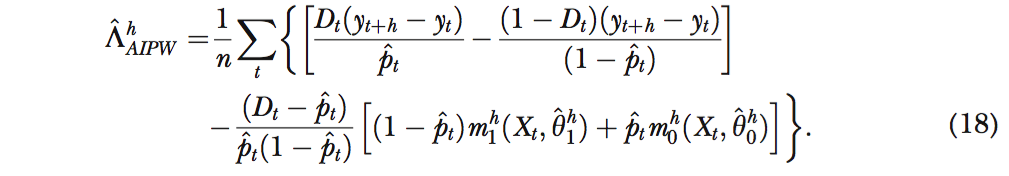
\includegraphics[scale=0.30]{eq18}}

\end{frame}
	
\begin{frame}{Changes in idiosyncratic risk}
	\begin{itemize}
	
	\item {
	As the unemployment insurance increases and idiosyncratic risk decreases, the aggregates decrease and approach the values of the representative agent model. 
	}

	\item {
Hence, with an increasing $\mu$ savings tend to decrease on average.
	}

	\item {
Looking at the distribution of capital holdings gives us an even better picture.
	}	

	\end{itemize} 
\end{frame}
	
\begin{frame}{Changes in idiosyncratic risk}

	

distributional plot 
  \centering{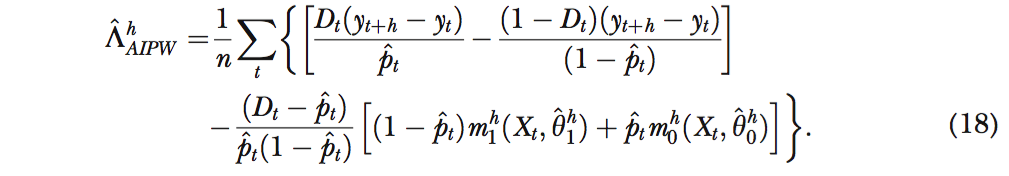
\includegraphics[scale=0.30]{eq18}}


\end{frame}


\begin{frame}{Changes in idiosyncratic risk}

\begin{itemize} 
	\item {
We saw that the policy change has a different effect on the unemployed and the employed. 
}
	\item {
Hence, we will now look at the different variables, to get an even better image.
}
\end{itemize}


\end{frame}






\begin{frame}{Changes in idiosyncratic risk}

	

big subplot with all the variables
  \centering{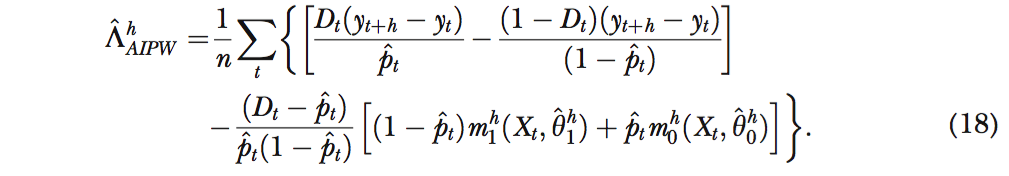
\includegraphics[scale=0.30]{eq18}}


\end{frame}

\begin{frame}{Changes in idiosyncratic risk}

	
We can distinguish between different effects: 

	\begin{itemize}
	\item {
The Income-effect: On aggregate consumers will have more income as unemployed receive additional benefits

	}	
	\item {
Tax-effect: The working are taxed to finance the unemployment benefits and to keep the government buget in balance, reducing their net-income. 

	}	
	\item {
Price effect: A reduction of individual risk by a more generous UI benefit decreases precautionary savings, and therefore reduces the aggregate capital stock. This will increase the interest rate and reduce the wage rate.
	}	

	\end{itemize} 
\end{frame}

\begin{frame}{Changes in idiosyncratic risk}
	
What conclusions can we draw from this?  

	\begin{itemize}
	\item {
There are diverse effects, affecting the agents' welfare in contradictory ways. Hence, we do need a different metric, in order to make qualified statements about the policy change. 
	}	
	\item {
The model neglegcts certain aspects: There is no voluntary unemployment. A change in the UI does not affect the overall unemployment rate, which contradicts empirical evidence. 
	}	
	\item {
Finally, it is important to note, that we only compare steady states. However, every policy change includes a transition phase, which might aversely affect the agents' welfare. 
	}	


	\end{itemize} 
\end{frame}


\section{Welfare effects}
\subsection{}


\section{Aggregate risk}
\subsection{}

\section{Conclusions}
\subsection{}

\end{document}